\section{Vermittlung}

\paragraph{Vermittlungstechniken --- Leitungsvermittlung}
\begin{items}
  \item \textbf{Prinzip}: Verbindung erhält \emph{durchgehenden Kanal} mit konstanter Bandbreite für exklusive Nutzung
  \item \textbf{Multiplexing}: \emph{starres Multiplexing} möglich \\*
    - \emph{Frequenzmultiplex}: Feste Zuweisung von Übertragungskanal + Frequenzabschnitt \\*
    - \emph{Zeitmultiplex}: Feste Zuweisung von Übertragungskanal + Zeitschlitz (\emph{time slot})
  \item \textbf{Eigenschaften}: \\*
    - Aufbau eines durchgehenden Übertragungskanals zwischen Endsystemen \\*
    - keine Adressinformation nötig, dafür Zustandshaltung \\*
    - zugesicherte, feste Datenrate \( \leadsto \) ungenutzte Ressourcen bei Nichtverwendung \\*
    - Übertragungsverzögerungen nur physikalisch bedingt \\* \phantom{-} \phantom{-} \( \leadsto \) keine Schwankungen durch Puffer \\*
    - Reihenfolgentreue Bitfolgenübertragung
  \item \textbf{Einsatzgebiete}: Telefonnetze, GSM
\end{items}

\paragraph{Vermittlungstechniken --- Paketvermittlung}
\begin{items}
  \item \textbf{Prinzip}: Weiterleitung anhand von Kontrollinformation in Paket \\*
    - Zieladresse in Datagrammen \\*
    - lokale Kennung bei virtuellen Verbindungen \\*
    - Zwischensysteme Speichern Pakete in \emph{Warteschlangen} \( \leadsto \) Paketverlust möglich
  \item \textbf{Eigenschaften}: \\*
    - Wechselnde Paketwege möglich \( \leadsto \) Reihenfolgevertauschung möglich \\*
    - Üblicherweise Zeitmultiplex
  \item \textbf{Varianten}: \\*
    - \emph{verbindungslos}: Datagramme \\*
    - \emph{verbindungsorientiert}: virtuelle Verbindungen
\end{items}
\begin{figure}[H]\centering\label{Paketvermittlung}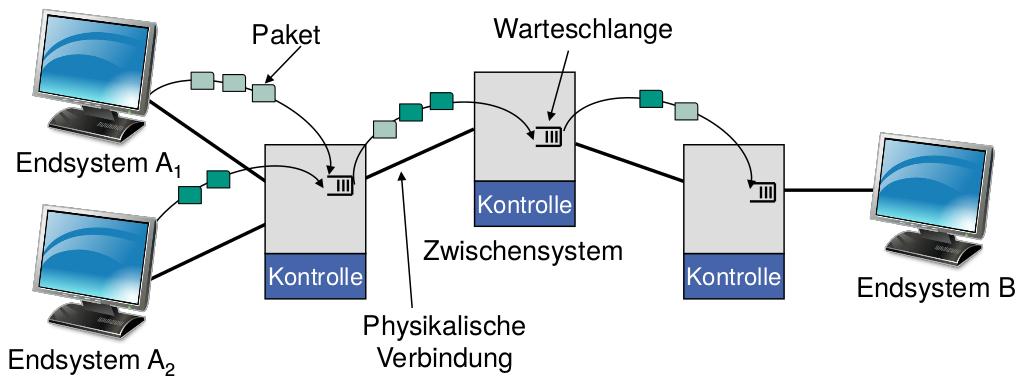
\includegraphics[width=0.33\textwidth]{Paketvermittlung}\end{figure}

\paragraph{Paketvermittlung --- Datagramme}
\begin{items}
  \item Pakete (= Datagramme) werden als isolierte Einheiten betrachtet
  \item \textbf{Ziel}: In jedem Datagramm enthalten \( \leadsto \) keine Verbindungsverwaltung nötig
  \item \textbf{Routing}: können Netz unterschiedlich durchlaufen \\*
    \( \leadsto \) Datagramme können bei Empfänger unsortiert ankommen
\end{items}

\paragraph{Paketvermittlung --- virtuelle Verbindungen}
\begin{items}
  \item fester Übertragungsweg zwischen zwei Endsystemen
  \item \textbf{Reihenfolgetreue}: Alle Pakete gehen selben Weg
  \item \textbf{Kennungen}: \emph{virtual circuit identifier} (VCI) kennzeichnen Pakete
  \item \textbf{Ziel}: Zieladresse nur bei Verbindungsaufbau nötig
  \item \textbf{Prozess}: Verbindungsaufbau \( \to \) Datenübertragung \( \to \) Verbindungsabbau
\end{items}

\paragraph{Vermittlungstechniken --- Nachrichtenvermittlung}
\begin{items}
  \item \emph{Vermittlung von Anwendungsnachrichten}
  \item Vermittlung üblicherweise mittels mehrerer Pakete \\*
    \( \leadsto \) \emph{Segmentierung} und \emph{Reassemblierung}
  \item \textbf{Zwischensysteme}: Reassemblierung nötig, da alle Teile in selbe Richtung weitergeleitet werden müssen
  \item \( \leadsto \) \emph{Ende-zu-Ende-Verzögerung wesentlich höher als bei Paketvermittlung}
\end{items}

\paragraph{Vermittlungsschicht --- Überblick}
\begin{items}
  \item \textbf{Ende-zu-Ende}: transportiert Segmente zwischen Endsystemen
  \item \textbf{Sender}: kapselt Segmente in Datagramme
  \item \textbf{Empfänger}: Segmente werden an Transportschicht ausgeliefert
  \item \textbf{Protokolle}: in \emph{allen} Endsystemen und Routern
  \item \textbf{Router}: werten Felder im Kopf aller Datagramme aus, die sie passieren
\end{items}

\paragraph{Vermittlungsschicht --- Aufgaben}
\begin{items}
  \item \textbf{Weiterleitung} (\emph{forwarding}): Datenebene \\*
    - Pakete werden von Routereingang an geeigneten Ausgabe weitergeleitet
  \item \textbf{Wegewahl} (\emph{routing}): Kontrollebene \\*
    - ermittelt Weg, den Pakete zurücklegen (sollen) \\*
    - erfordert Routingalgorithmus + -protokoll
\end{items}

\paragraph{Vermittlungsschicht --- Kontroll- und Datenebene}
\begin{items}
  \item \textbf{Kontrollebene}: \\*
    - betrachtet gesamtes Netz \\*
    - bestimmt wie Datagramm über Router von Quelle zu Ziel geroutet wird \\*
    - \emph{Konzepte}: \\
    \phantom{-} \( \cdot \) traditionelle Routingalgorithmen: in jedem Router implementiert \\*
    \phantom{-} \( \cdot \) \emph{software defined networking} (SDN): in logisch zentralen Servern implementiert
  \item \textbf{Datenebene}: \\*
    - Funktionen lokal in Router \\*
    - Bestimmt wie Datagramm von Eingangs- zu Ausgangsport geleitet wird
\end{items}

\paragraph{Vermittlungsschicht --- Begriffe}
\begin{items}
  \item \textbf{Router}: \\*
    - auf Vermittlungsschicht operierendes Zwischensystem \\*
    - leitet Datagramme mithilfe von Weiterleitungstabelle weiter \\*
    - tauscht über Routingprotokolle Informationen mit anderen Routern aus
  \item \textbf{Route}: Weg eines Datagramms von Start zu Ziel
  \item \textbf{Link}: Übertragungsabschnitt zwischen 2 Routern (kann z.B. auch Brücken enthalten)
  \item \textbf{Port}: Eingangs-/Ausgangs-Netzwerkschnittstelle
\end{items}

\paragraph{Vermittlungsschicht --- Protokolle}
\begin{items}
  \item \textbf{IP} (\emph{internet protocol}): \\*
    unzuverlässige Datagrammübertragung
  \item \textbf{ICMP} (\emph{internet control message protocol}): \\*
    Kontrollinformationsaustausch innerhalb der Vermittlungsschicht
  \item \textbf{ARP} (\emph{address resolution protocol}): \\*
    Zuordnung von IP-Adressen zu Adressen der Sicherungsschicht
  \item \textbf{RARP} \emph{reverse ARP}: \\*
    Umkehrfunktionen von ARP
  \item \textbf{BGP} (\emph{border gateway protocol}), \textbf{RIP} (\emph{routing information protocol}), \textbf{OSPF} (\emph{open shortest path first}): Routingprotokolle
\end{items}

\paragraph{Vermittlung --- IP}
\begin{items}
  \item IP macht die ganze Vermittlung \( \leadsto \) nur ein großes Vermittlungsprotokoll \\*
    - Interoperabilität erhöhen \\*
    - Anzahl unterschiedlicher Interfaces erniedrigen \\*
    - kleinster gemeinsamer Nenner \\*
    - Anzahl nutzbarer Netze maximieren
\end{items}
\begin{figure}[H]\centering\label{IP}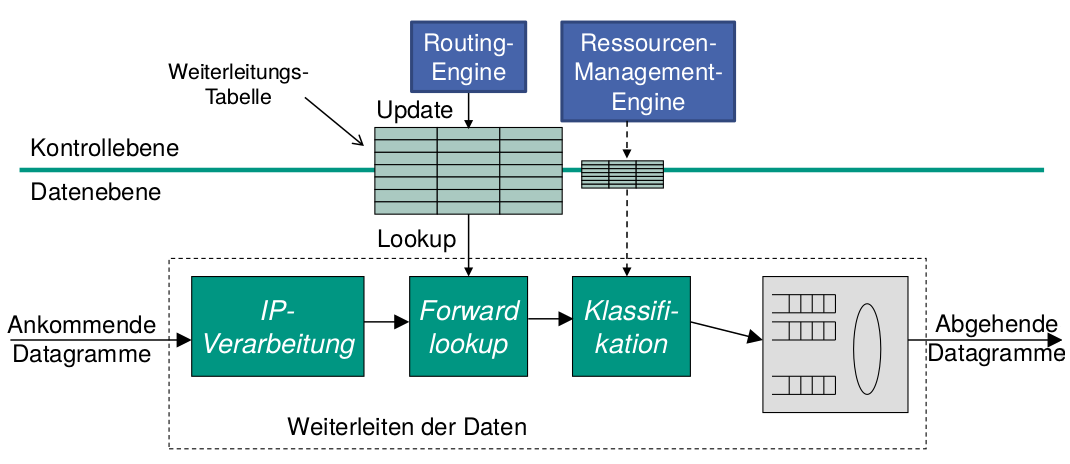
\includegraphics[width=0.4\textwidth]{IP}\end{figure}

\paragraph{IP --- Fragementieren + Reassemblieren}
\begin{items}
  \item Anpassung an Maximallänge unterliegender Netze (\textbf{MTU}: \emph{maximum transfer unit})
  \item \textbf{Flag-Felder} IP-Kopf: \\*
    - \emph{Bit 0}: reserviert, muss 0 sein \\*
    - \emph{Bit 1}: 0 = darf fragmentiert werden, 1 = nicht \\*
    - \emph{Bit 2}: 0 = letztes Fragment, 1 = nicht
\end{items}

\paragraph{IP --- Weiterleitung}
\begin{items}
  \item \textbf{Endsystem}: \\*
    - Rechner mit Zieladresse direkt verbunden \( \to \) Datagramm direkt zustellen \\*
    - Sonst: Datagramm-Übergabe an Standardrouter
  \item \textbf{Router}: Verwendung \emph{Weiterleitungstabelle} \\*
    - \emph{Zieladresse} \\*
    - \emph{Next-Hop-Router} \\*
    - \emph{Flags}, die Start und Ziel genauer klassifizieren \\*
    - \emph{Netzschnittstelle}, auf die bei Endsystem das Datagramm ausgegeben werden soll
  \item \textbf{Weiterleitungstabelle}: Identifikation des nächsten Systems auf Weg zum Ziel
\end{items}

\paragraph{IP --- Empfangsprozess}
\begin{items}
  \item \textbf{Überprüfungen}: \\* 
    - \emph{Kopflänge} \\*
    - \emph{Datagrammlänge} \\*
    - \emph{Versionsnummer} IP \\*
    - \emph{Prüfsumme} \\*
    - \emph{Lebenszeit} \\*
    - \emph{Protokoll-Identifikation} \\*
    - \emph{Adressklassen}
  \item \textbf{Fehlerfall}: Benachrichtigung ICMP (\emph{internet control message protocol}) --- möglicherweise wird ICMP-Paket ausgesendet
\end{items}

\paragraph{IP --- Adressierung}
\begin{items}
  \item \textbf{Ziel}: Eindeutige Identifizierung aller angeschlossenen Systemschnittstellen
  \item \textbf{IP-Adressen}: Kennungen für Interfaces von Routern/Endsystemen \\*
    - \emph{IPv4}: 32 Bit-Adressen \\*
    - \emph{IPv6}: 128 Bit-Adressen
\end{items}

\paragraph{IP --- Subnetze}
\begin{items}
  \item \textbf{Gliederung}: IP-Adresse unterteilt in \\*
    - \emph{Subnetz-Teil}: high order bits \\*
    - \emph{Endsystem-Teil}: low order bits
  \item \textbf{Subnetz}: Interfaces mit selbem Subnetz-Teil, können ohne Router kommunizieren
\end{items}

\paragraph{Adresszuteilung}
\begin{items}
  \item \textbf{Manuell}: Durch Systemadministrator
  \item \textbf{Dynamisch}: \emph{dynamic host configuration protocol} (DHCP) \\*
    - DHCP-Server liefert IP auf Anfrage
\end{items}

\paragraph{Adressblockzuteilung}
\begin{items}
  \item \textbf{Provider}: Erhält Block von \textbf{ICANN} (\emph{internet corporation for assigned names/numbers}) \\*
    - ICANN allokiert Adressen \\*
    - ICANN verwaltet DNS \\*
    - ICANN weist Domainnamen zu
\end{items}

\paragraph{Internet Control Message Protocol (ICMP)}
\begin{items}
  \item \textbf{Einzelne Datagrammverluste}: meldet IP nicht (unzuverlässiger Dienst)
  \item \textbf{Schwerwiegende Probleme} (z.B. Verbindungsabbruch): Mitteilung an Kommunikationspartner via ICMP
  \item \( \Rightarrow \) ICMP tauscht Fehlernachrichten, Statusanfragen und Zustandsinformationen aus
\end{items}

\paragraph{ICMP --- Statusanfragen}
\begin{items}
  \item \textbf{Echo + Antwort} (\emph{echo and echo reply}): \\*
    - Aktivitätsüberprüfung von Kommunikationssystemen \\*
    - Empfänger von Echo-Anfrage sendet erhaltene Daten in Echo-Antwort zurück
  \item \textbf{Zeitstempel + Antwort} (\emph{timestamp and timestamp reply}): \\*
    - Bestimmung von Umlaufzeiten (\emph{round trip time}, RTT) \\*
\end{items}

\paragraph{IPv6}
\begin{items}
  \item \textbf{Problem}: \\*
    - Adressraum von IPv4 geht aus \\*
    - Kopfformat IPv4 nicht optimal
  \item \textbf{Lösung}: \\*
    - Erhöhung Adresslänge von 32 auf 128 Bit \\*
    - feste Kopflänge (40 Byte) \\*
    - keine Unterstützung von Fragmentierung \\*
    - keine Prüfsumme \\*
    - Optionen: als Erweiterungsköpfe (\emph{next header}) \\*
    - ICMPv6: neue Version von ICMP
\end{items}

\paragraph{Routing --- Prinzipien}
\begin{items}
  \item \textbf{Ziel}: guten Weg durch Netz finden
  \item \textbf{Weg}: Sequenz von Routern von Start- zu Ziel-Endsystem
  \item \textbf{Netzgraph}: Netz wird als Graph verstanden \\*
    - \emph{Knoten}: Router \\*
    - \emph{Kanten}: Übertragungsabschnitte (Kantenkosten z.B. Verzögerung, Preis,\dots) \\*
  \item \textbf{Pfad}: Knotenfolge (meist Pfad mit kürzester Länge gesucht)
\end{items}

\paragraph{Routing-Verfahren --- Dynamik}
\begin{items}
  \item \textbf{Frage}: Wie dynamisch ist Routing-Verfahren?
  \item \textbf{Nicht adaptiv}: Routen ändern sich sehr selten, wesentlich seltener als \\* Verkehrsänderungen
  \item \textbf{Adaptiv}: \\*
    - Routen ändern sich abhängig von Verkehr und Topologie \\*
    - Routenänderungen periodisch oder reaktiv \\*
    - \emph{Zielkonflikt}: Systeme haben ggf kein Live-Abbild des Netzes \\*
      \phantom{-} \phantom{\( \cdot \)} ggf hohe Netzbelastung durch Routing-Informationsaustausch
\end{items}

\paragraph{Routing-Verfahren --- statisches Routing}
\begin{items}
  \item \textbf{Beispiel}: \\*
    - Zufallszahl \( 1 < x \leq 0 \) \\*
    - Falls \( x < 0.6 \) weiterleiten nach B \\*
    - Falls \( 0.9 \geq x \geq 0.6 \) weiterleiten nach C \\*
    - Sonst D
\end{items}

\paragraph{Routing-Verfahren --- zentralisiert}
\begin{items}
  \item Adaptives Verfahren
  \item \textbf{Routing Control Center}: Für Berechnung/Verteilung der optimalen Pfade \\*
    - Systeme senden periodisch Zustand an RCC \\* \phantom{-} \phantom{\( \cdot \)} (aktive Nachbarn, Warteschlangenlängen,\dots)
  \item \textbf{Vorteile}: \\*
    - RCC hat alle Informationen \( \leadsto \) kann perfekte Entscheidungen treffen \\*
    - Systeme müssen kein Routing betreiben
  \item \textbf{Nachteile}: \\*
    - Berechnungsdauer für große Netze ggf sehr lang \\*
    - Ausfall RCC lähmt ganzes Netz \\*
    - Inkonsistenzen möglich, da Systeme nah an RCC Tabellen schneller erhalten \\*
    - starke Belastung des RCC
\end{items}

\paragraph{Routing-Verfahren --- isoliert}
\begin{items}
  \item \textbf{Prinzip}: Jedes System entscheidet anhand selbstgesammelter Information \\*
    - kein Routinginformationsaustausch zwischen Systemen
\end{items}

\paragraph{Isoliertes Routing --- Fluten}
\begin{items}
  \item \textbf{Prinzip}: Jedes eingehende Datagramm wird auf jeder Übertragungsleitung weitergeleitet
  \item \textbf{Fluteindämmung}: \\*
    - \emph{Sequenznummern} für Duplikaterkennung \\*
    - \emph{Lebensdauerkontrolle} durch Zählen der Übertragungsabschnitte (\emph{hops}) \\*
  \item \textbf{Varianten}: \\*
    - \emph{selektives Fluten}: Weiterleitung nicht auf allen Übertragungsabschnitten \\*
    - \emph{random walk}: Zufällige Auswahl eines Übertragungsabschnittes
\end{items}

\paragraph{Isoliertes Routing --- Hot Potato}
\begin{items}
  \item \textbf{Prinzip}: Jeder versucht Datagramme so schnell wie möglich weiterzuleiten \\*
    \( \leadsto \) Übertragungsabschnitt mit kürzester Warteschlange wählen
  \item \textbf{Varianten}: \\*
    - nie an Herkunftsleitung weiterleiten \\*
    - Kombination mit statischem Routing: statisches Verfahren zur Auswahl von \\* \phantom{-} \phantom{\( \cdot \)} Leitung mit Warteschlangenlänge unter Schwellwert
\end{items}

\paragraph{Routing-Verfahren --- Verteiltes adaptives Routing}
\begin{items}
  \item \textbf{Prinzip}: Systeme tauschen Routing-Informationen mit Nachbarn aus \\*
    - jedes System unterhält Routing-Tabelle
  \item \textbf{Varianten}: \\*
    - periodischer Informationsaustausch \\*
    - Austausch nur bei größeren Änderungen
\end{items}

\paragraph{Routing-Algorithmen --- Übersicht}
\begin{items}
  \item \textbf{Distanz-Vektor-Algorithmen}: Distanz als Routing-Metrik \\*
    - jeder Router kennt Distanz zu allen anderen Systemen im Netz \\*
    - \emph{Problem}: kürzerer langsamer Weg wird längerem schnelleren vorgezogen
  \item \textbf{Link-State-Algorithmen}: Unterschiedliche Routing-Metriken \\*
    - berücksichtigt aktuelle Zustände der Netzanschlüsse \\*
    - jeder Router kennt ganze Netztopologie \\*
    - Link-State- konvergieren schneller als Distanz-Vektor-Algorithmen \\* 
\end{items}

\paragraph{Routing-Algorithmen --- Distanz-Vektor}
\begin{items}
  \item \textbf{Eigenschaften}: \\*
    - \emph{verteilt}: jeder Router erhält Infos von direkten Nachbarn, führt Berechnung durch \\* \phantom{-} \phantom{\( \cdot \)} und verteilt dann neue Informationen an direkte Nachbarn \\*
    - \emph{iterativ}: Verteilen + Berechnen von Informationen so lange, bis keine Information \\* \phantom{-} \phantom{\( \cdot \)} mehr ausgetauscht wird
  \item \textbf{Distanz-Vektor-Tabelle}: \\*
    - Grundlegende, in jedem System vorhandene Datenstruktur \\*
    - Zeile für jedes mögliche Ziel \\*
    - Spalte für direkte Nachbarn \\*
\end{items}

\paragraph{Distanz-Vektor-Routing --- Distanz-Vektor-Tabelle}
\begin{items}
  \item \textbf{Beispiel}: \( X \) will Daten über direkten Nachbar \( Z \) an \( Y \) weiterleiten \\*
    - \( D^X(Y,Z) = c(X,Z) + \underset{w}{\text{min}}\{ D^Z(Y,w) \} \)
  \item \textbf{Beispiel}: \( D^E(A,D) \) \\*
    - erster Übertragungsabschnitt: \( E \to D \) \\*
    - Tabelleneintrag: Kosten \( E \to D \) (\( =2 \)) + minimale Kosten \( D \to A \) (\( =3 \)) \\*
    \phantom{-} \( \leadsto \) \textbf{minimale Kosten von \( D \) nach \( A \) über Nachbar von \( D \)}
\end{items}
\begin{figure}[H]\centering\label{DistanzVektor}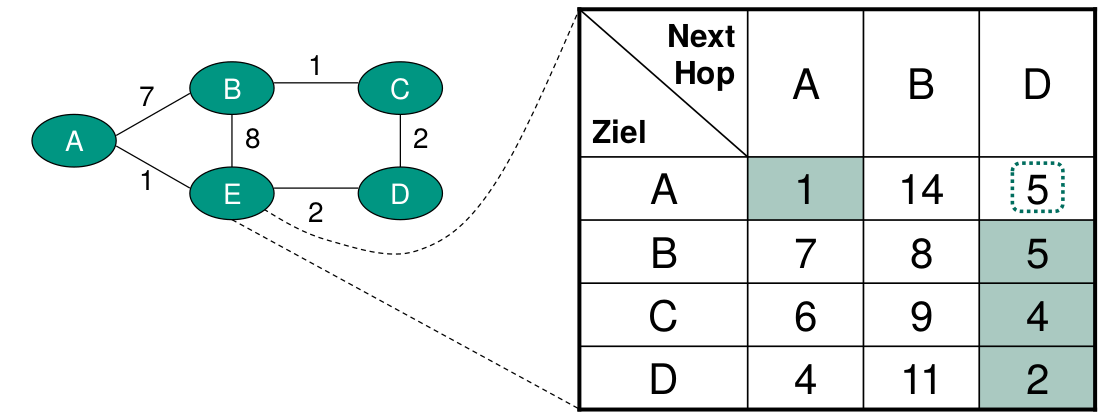
\includegraphics[width=0.4\textwidth]{DistanzVektor}\end{figure}

\paragraph{Distanz-Vektor --- Distanz-Vektor-Algorithmus (Bellman-Ford)}
\begin{items}
  \item \textbf{Initialisierung}: \\*
    - für alle Nachbarn \( v \): \( D^X(*,v) = \infty \), \( D^X(v,v) = c(X,v) \) \\*
    - für alle Ziele \( y \): sende \( \underset{w}{\text{min}}D^w(y,w) \) allen Nachbarn (\( w \) enthält alle Nachbarn)
  \item \textbf{Schleife}: \\*
    - geänderte Abschnittskosten: für alle Ziele \( y \): \( D^X(y,V) \coloneqq D^X(y,V) + d \) \\*
    - Update von Nachbarn: kürzester Pfad von \( V \) zu Ziel \( Y \) hat sich um \( \alpha \) geändert \\*
    \phantom{-} \( \leadsto \) \( D^X(Y,V) \coloneqq c(X,V) + \alpha \) \\*
    \phantom{-} \( \leadsto \) Falls neuer \( \underset{w}{\text{min}}D^w(Y,w) \) für Ziel \( Y \) existiert, dann sende allen direkten \\* \phantom{-} \phantom{\( \leadsto \)} Nachbarn diesen Wert
  \item \textbf{Komplexität}: \( O(n^2k) \) für \( n \) Knoten und \( k \) Kanten
\end{items}

\paragraph{Distanz-Vektor-Algorithmus --- Updateausbreitung}
\begin{items}
  \item \textbf{Ausbreitung good news}: schnelle Ausbreitung
  \item \textbf{Ausbreitung bad news}: langsame Ausbreitung, ggf Routing-Schleifen \\*
    \( \leadsto \) \textbf{Count to Infinity-Problem}
\end{items}

\paragraph{Distanz-Vektor-Algorithmus --- poisoned reverse}
\begin{items}
  \item \textbf{Ziel}: Vermeidung von Routing-Schleifen
  \item \textbf{Prinzip}: Routing-Information wird \( Y \) vorenthalten, wenn Weg über \( Y \) kürzer
\end{items}

\paragraph{Routing-Algorithmen --- Link-State-Routing}
\begin{items}
  \item \textbf{Prinzip}: \\*
    - Systeme müssen zu Beginn nur direkte Nachbarn kennen \\*
    - Entdecken von neuen Nachbarn zB mittels \code{HELLO}-Pakete \\*
    - \emph{link state broadcast}: Identität + Kosten zu Nachbarn werden allen Routern im Netz \\* \phantom{-} \phantom{\( \cdot \)} weitergeleitet (Fluten) \\*
    - Systeme lernen Topologie durch LSBs der anderen Systeme \\*
    - \emph{Ergebnis}: Alle Systeme haben \emph{identisches} Wissen über Netz
  \item \textbf{Implementierung}: Dijkstra-Algorithmus
\end{items}

\paragraph{Link-State vs. Distanz-Vektor}
\begin{items}
  \item \textbf{Komplexität Kontroll-Pakete}: \\*
    - \emph{link-state}: jedes System muss Kosten aller Links kennen, Änderungen müssen an \\* \phantom{-} \phantom{\( \cdot \)} alle Systeme geschickt werden \\*
    - \emph{Distanz-Vektor}: Änderungen nur an benachbarte Systeme weitergegeben
  \item \textbf{Konvergenzgeschwindigkeit}: \\*
    - \emph{link-state}: \( O(n^2) \), \( O(nE) \) Pakete \( \leadsto \) schnelle Konvergenz, danach schleifenfrei, \\* \phantom{-} \phantom{\( \cdot \)} aber Oszillationen möglich \\*
    - \emph{Distanz-Vektor}: langsame Konvergenz, Schleifen möglich, Count-to-Infinity kann \\* \phantom{-} \phantom{\( \cdot \)} auftreten
  \item \textbf{Robustheit}: \\*
    - \emph{link-state}: Routenberechnungen separiert \( \leadsto \) Robustheit \\*
    - \emph{Distanz-Vektor}: ein System kann inkorrekte Pfade zu allen Zielen verbreiten
  \item \textbf{Gewinner?} \\*
    - \emph{link-state}: Konvergiert schneller, ist robuster \\*
    - \emph{Distanz-Vektor}: einfacher zu implementieren
\end{items}

\paragraph{software defined networking}
\begin{items}
  \item \textbf{Eigenschaften}: \\*
    - \textbf{E1}: Separierung von Kontroll- und Datenebene \\*
    - \textbf{E2}: Flow-basierte Paketweiterleitung \\*
    - \textbf{E3}: Log an externen Controller ausgelagert \\*
    - \textbf{E3}: Netzwerk programmierbar
  \item \textbf{Umsetzung}: \emph{open flow}-Protokoll \\*
    - regelt Kommunikation zwischen Controller und Switch \\*
    - OpenFlow quasi-Standard, Alternativen existieren
\end{items}

\paragraph{Traditionelles IP-Routing}
\begin{items}
  \item Kontroll- und Datenebene in jedem Router
  \item \textbf{Vorteile}: \\*
    - Ausfallsicherheit (selbstorganisiert, verteilte Kontrolle, hohe Redundanz) \\*
    - Schnelle Reaktion (optimierte Routing-Hardware, lokale Routingentscheidung) \\*
    - Bewährtes Konzept
  \item \textbf{Nachteile}: \\*
    - proprietäre Management-Schnittstellen (Mischbetrieb schwierig) \\*
    - unflexibel (neue Funktionen hinzufügen schwierig, aufwändige Standardisierung) \\*
    - teuer (hochqualifiziertes Personal + Overprovisioning benötigt)
\end{items}
\begin{figure}[H]\centering\label{IPRoutingTraditionell}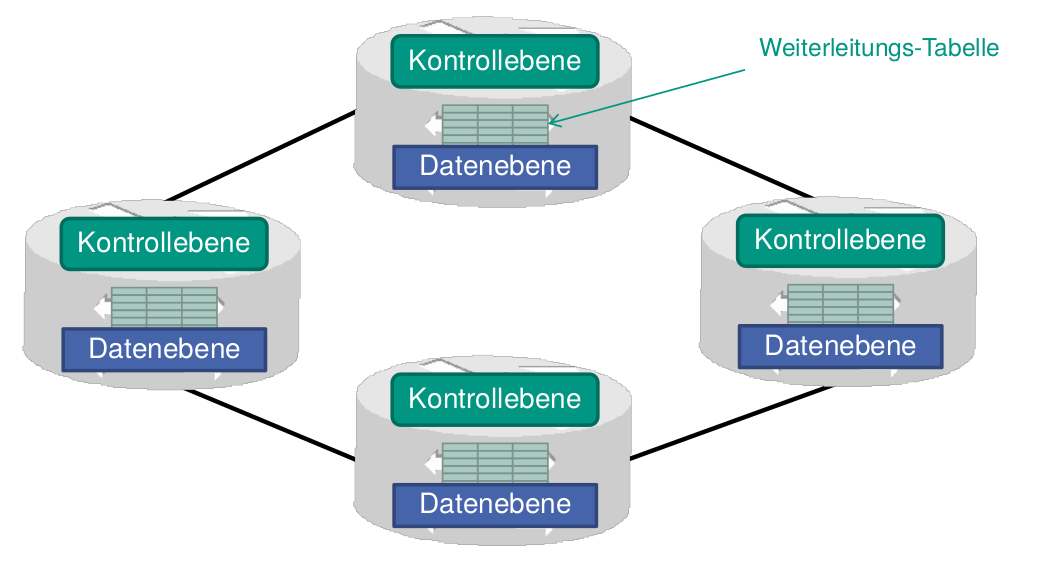
\includegraphics[width=0.33\textwidth]{IPRoutingTraditionell}\end{figure}

\paragraph{SDN-Routing}
\begin{items}
  \item \textbf{Vorteile}: \\*
    - logisch zentralisierte Sicht (Controller hat Netzüberblick, einfacher Einsatz von \\* \phantom{-} \phantom{\( \cdot \)} Graphalgorithmen) \\*
    - neue Funktionalität in Software (als App im Controller \\* \phantom{-} \phantom{\( \cdot \)} \( \leadsto \) kürzere Entwicklungszyklen) \\*
    - Trennung von Kontroll- und Datenebene (Innovationen unabhängig möglich, \\* \phantom{-} \phantom{\( \cdot \)} herstellerunabhängig durch offene Schnittstellen)
  \item \textbf{Nachteile}: \\*
    - Skalierbarkeit \\*
    - \emph{single point of failure} \\*
    - Kommunikation mit Controller langsam
\end{items}
\begin{figure}[H]\centering\label{SDNRouting}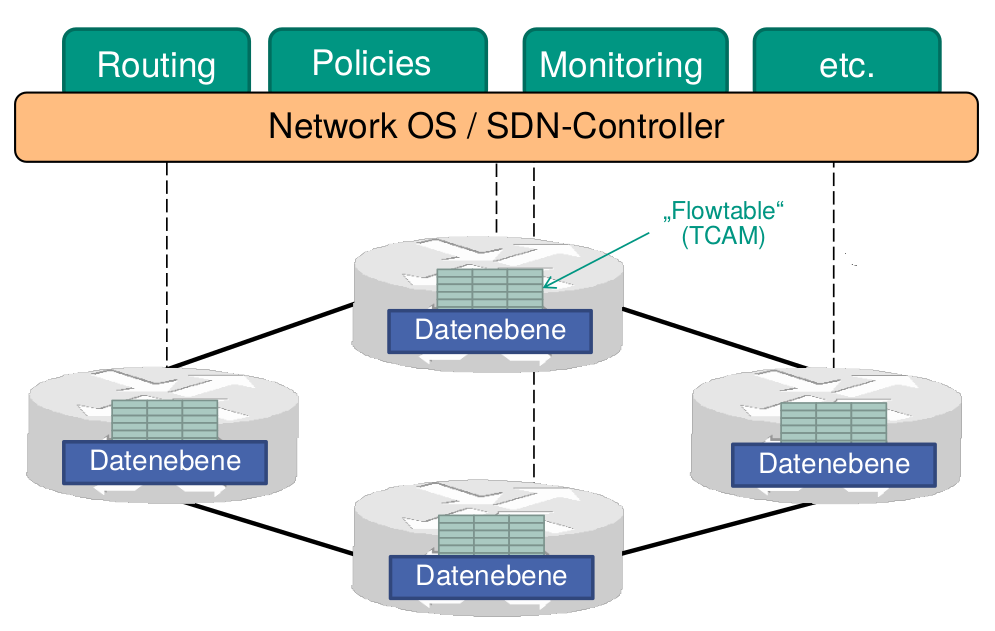
\includegraphics[width=0.33\textwidth]{SDNRouting}\end{figure}

\paragraph{SDN --- Traditioneller Router vs. SDN-Switch}
\begin{items}
  \item \textbf{Traditioneller IP-Router}: \\*
    - kennt keine Flows \\*
    - Weiterleitung über Ziel-IP-Adresse
  \item \textbf{SDN-Switch}: \\*
    - Weiterleitung über Flowtable \\*
    - nutzt verschiedene IP-Kopf-Felder \\*
    - speichert Zustand pro Flow
\end{items}
\begin{figure}[H]\centering\label{SDNFlow}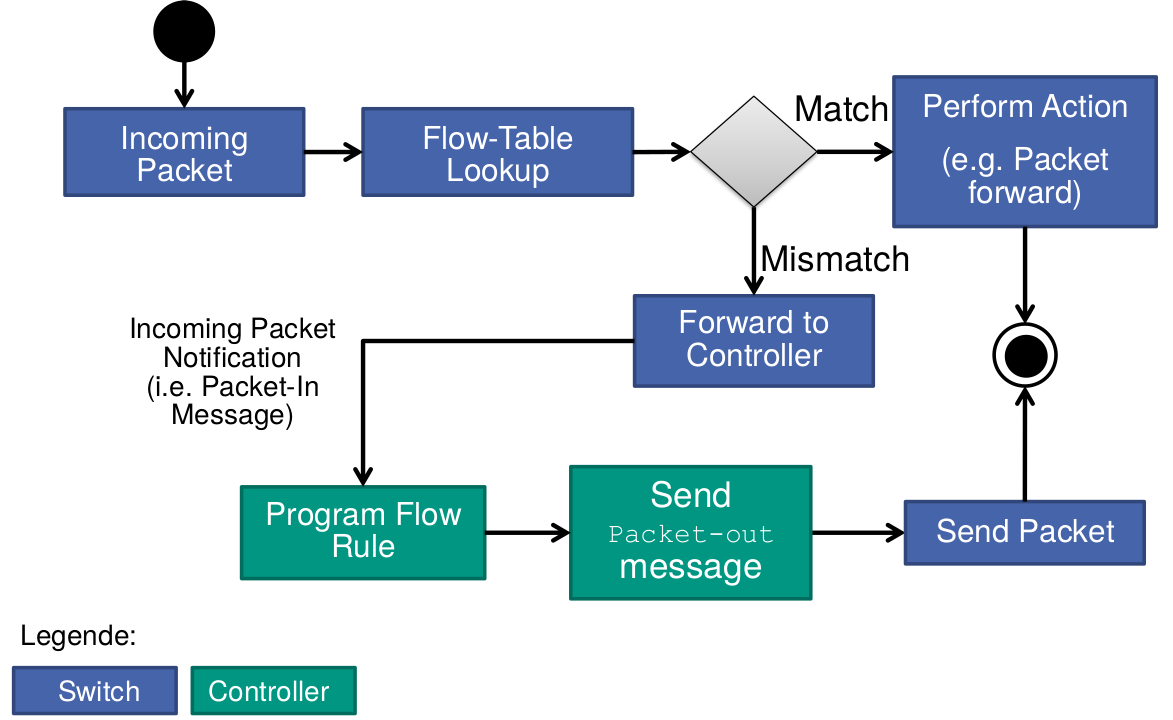
\includegraphics[width=0.33\textwidth]{SDNFlow}\end{figure}